\subsubsection{Scenario S1: Il contributore attivo}

Lo Scenario S1 ha richiesto agli utenti di simulare un contesto realistico in cui, in seguito al superamento di un esame, si mettono a disposizione i propri appunti impostando come ``Pubblico'' un file precedentemente caricato. Successivamente, l'obiettivo prevedeva la creazione di un nuovo esame denominato ``Fondamenti di Informatica'', l'esplorazione della community per individuare appunti relativi a tale corso e, infine, l'associazione diretta del materiale individuato all'esame appena pianificato.

\paragraph{Analisi delle prestazioni generali}

Come si può notare dai dati aggregati per lo Scenario S1 (Tabella~\ref{tab:6-s1-1}), il tasso di completamento (\textit{Success Rate}) si è attestato al 100,00\% per entrambe le versioni del sistema. L'analisi dei dati globali aggregati per questo scenario complesso restituisce un quadro inequivocabile dell'impatto positivo della riprogettazione. Pur mantenendo un tasso di completamento (\textit{Success Rate}) invariato al 100,00\% in entrambe le varianti, la versione post-riprogettazione (B) ha generato un sensibile abbattimento del 54,84\% nella media degli errori, passata da 2,21 a 1,00. Contestualmente, si registra una decisa contrazione del 41,82\% nella mediana dei click (da 55 a 32) e una riduzione del 14,86\% nella mediana del tempo di esecuzione (da 4:36 a 3:55). Risulta particolarmente indicativa anche la diminuzione della difficoltà percepita, che cala del 36,36\%, passando da 3,67 a 2,33.

\begin{figure}[H]
	\centering
	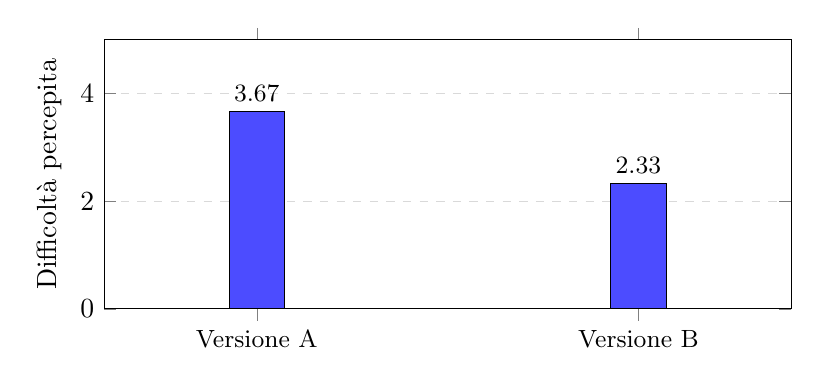
\begin{tikzpicture}
		\begin{axis}[
				ybar,
				bar width=20pt,
				width=0.85\textwidth,
				height=5cm,
				symbolic x coords={Versione A, Versione B},
				xtick=data,
				x tick label style={font=\small},
				ylabel={Difficoltà percepita},
				ymin=0, ymax=5,
				ymajorgrids=true,
				grid style={dashed, gray!30},
				enlarge x limits=0.4,
				nodes near coords,
				every node near coord/.style={font=\small, color=black},
			]
			\addplot+[
				ybar,
				fill=blue!70,
				draw=black
			] coordinates {
					(Versione A,3.67)
					(Versione B,2.33)
				};
		\end{axis}
	\end{tikzpicture}
	\caption{Confronto della difficoltà percepita tra Versione A e Versione B per S1.}
	\label{fig:6-s1-1}
\end{figure}

\begin{table}[H]
	\centering
	\footnotesize
	\renewcommand{\arraystretch}{1.2}
	\caption{Metriche prestazionali globali aggregate per lo Scenario S1.}
	\label{tab:6-s1-1}
	\begin{tabular}{|>{\raggedright\arraybackslash}p{2.2cm}|>{\centering\arraybackslash}p{1.5cm}|>{\centering\arraybackslash}p{1.5cm}|>{\centering\arraybackslash}p{1.5cm}|>{\centering\arraybackslash}p{1.5cm}|>{\centering\arraybackslash}p{1.8cm}|>{\centering\arraybackslash}p{1.6cm}|}
		\hline
		\rowcolor{gray!30}
		\textbf{S1}           & \multicolumn{2}{c|}{\textbf{Versione A}} & \multicolumn{2}{c|}{\textbf{Versione B}} & \textbf{Variazione \%} & \textbf{Rilevanza}                                            \\ \hline
		\textit{Success Rate} & \multicolumn{2}{c|}{100,00\%}            & \multicolumn{2}{c|}{100,00\%}            & \textbf{Invariato}     &                                                               \\ \hline
		\rowcolor{gray!30}
		                      & \textbf{Media}                           & \textbf{DEV.ST}                          & \textbf{Media}         & \textbf{DEV.ST}    & \multicolumn{2}{c|}{}                    \\ \hline
		\textit{Errori}       & 2,21                                     & 2,00686                                  & 1,000                  & 1,06904            & \textbf{-54,84\%}     & \pvalue{0,00244} \\ \hline
		\textit{Tempo}        & 4.55.16                                  & 0,09028                                  & 4.13.04                & 0,05625            & \textbf{-14,29\%}     & \pvalue{0,13855} \\ \hline
		\textit{Click}        & 53,33                                    & 13,62596                                 & 27,73                  & 8,20685            & \textbf{-48,00\%}     & \pvalue{0,00001} \\ \hline
		\rowcolor{gray!30}
		                      & \multicolumn{2}{c|}{\textbf{Mediana}}    & \multicolumn{2}{c|}{\textbf{Mediana}}    & \multicolumn{2}{c|}{}                                                                  \\ \hline
		\textit{Difficoltà}   & \multicolumn{2}{c|}{4}                   & \multicolumn{2}{c|}{2}                   & \multicolumn{2}{c|}{}                                                                  \\ \hline
	\end{tabular}
\end{table}

La riduzione degli errori e il dimezzamento del numero di click (23 in meno nella mediana) mostrano che la riprogettazione ha reso il flusso di lavoro più chiaro ed efficiente. Gli utenti hanno potuto completare le operazioni con meno passaggi inutili e con minori difficoltà.

\paragraph{Analisi qualitativa: commenti e osservazioni degli utenti}

L'elevato numero di errori e click registrato nella versione originale (A) trova conferma nelle osservazioni qualitative raccolte durante i test, che evidenziano diversi problemi legati all'organizzazione e alla comprensibilità dell'interfaccia:

\begin{itemize}
	\item \textbf{Disorientamento e terminologia poco chiara}: l'interfaccia originale è stata descritta dagli utenti come `tutto caotico, non si capisce dove bisogna andare''. In particolare, l'etichetta `StudyFlow AI'' utilizzata per la sezione degli esami è risultata poco intuitiva, tanto che molti partecipanti non l'hanno considerata come una possibile destinazione. Di conseguenza, gli utenti hanno dovuto cercare percorsi alternativi, passando dalla dashboard per creare un nuovo esame.


	\item \textbf{Mancanza di feedback e problemi di interazione}: l'inserimento dei dati è stato reso più difficile dall'assenza di messaggi chiari in caso di errore. Quando alcuni campi obbligatori (come dipartimento e ciclo di studi) non venivano compilati, il sistema non spiegava il motivo del mancato completamento dell'operazione. Ulteriore confusione è stata causata da valori preimpostati in alcuni \textit{listbox} e da aggiornamenti improvvisi della pagina durante l'inserimento delle informazioni.

	\item \textbf{Incoerenza linguistica}: la presenza contemporanea di elementi in italiano e in inglese, descritta dagli utenti come ``un po' italiano e un po' inglese'', ha contribuito ad aumentare il senso di disorientamento.
\end{itemize}

Per la versione post-riprogettazione (B), i commenti raccolti confermano invece un netto miglioramento dell'esperienza d'uso:

\begin{itemize}
	\item \textbf{Flusso più chiaro e organizzato}: l'interfaccia è stata valutata positivamente e descritta come ``molto condensato e facile da trovare ciò che cerco di fare''. Gli utenti sono riusciti a comprendere più facilmente il funzionamento del sistema, salvando correttamente i file e associandoli agli esami senza particolari difficoltà.

	\item \textbf{Possibili miglioramenti}: nonostante il flusso sia stato notevolmente semplificato, alcuni partecipanti hanno comunque definito l'interazione ``macchinosa'', sottolineando la necessità di spostarsi più volte tra sezioni diverse. Per questo motivo è stata suggerita l'introduzione di una scorciatoia che permetta di aggiungere direttamente gli appunti a un esame dalla sezione dei salvataggi personali o dalla community.

\end{itemize}

\paragraph{Valutazione dell'effetto di apprendimento}

Analizzando i dati in base all'ordine di esecuzione (Tabella~\ref{tab:6-s1-2}), emerge come una struttura più chiara dell'interfaccia favorisca l'apprendimento del compito da parte degli utenti.

Nel gruppo che ha utilizzato prima la versione A e poi la versione B, il primo approccio all'interfaccia originale ha richiesto un tempo mediano molto elevato, pari a 6:30. La presenza di percorsi poco chiari e di diversi elementi di confusione ha rallentato significativamente l'esecuzione del compito. Con il passaggio alla versione riprogettata (B), il tempo mediano si è ridotto del 37,18\%, scendendo a 4:05.

Il risultato più interessante emerge però dal gruppo che ha utilizzato le interfacce nell'ordine B--A. Gli utenti hanno impiegato inizialmente 3:47,5 per completare lo scenario nella versione riprogettata, apprendendo così la sequenza corretta delle operazioni. Una volta acquisita questa conoscenza, sono riusciti a completare lo stesso compito nella versione originale in soli 2:35,5.

Questo risultato suggerisce un forte effetto di \textit{transfer cognitivo}: la maggiore chiarezza della versione B ha aiutato gli utenti a costruire un modello mentale efficace del flusso di lavoro. Grazie a questa comprensione preliminare, sono stati in grado di orientarsi più facilmente anche nella versione originale, superandone le criticità e completando il compito in tempi molto inferiori rispetto agli utenti che avevano iniziato direttamente dalla versione A.

\begin{table}[H]
	\centering
	\footnotesize
	\renewcommand{\arraystretch}{1.2}
	\caption{Confronto delle metriche prestazionali in funzione dell'ordine di esecuzione per lo Scenario S1.}
	\label{tab:6-s1-2}
	\begin{tabular}{|>{\raggedright\arraybackslash}p{2.2cm}|>{\centering\arraybackslash}p{1.0cm}|>{\centering\arraybackslash}p{1.0cm}|>{\centering\arraybackslash}p{1.8cm}|>{\centering\arraybackslash}p{1.6cm}|>{\centering\arraybackslash}p{1.0cm}|>{\centering\arraybackslash}p{1.0cm}|>{\centering\arraybackslash}p{1.8cm}|>{\centering\arraybackslash}p{1.6cm}|}
		\hline
		\rowcolor{gray!30}
		\textbf{Metrica}              & \multicolumn{4}{c|}{\textbf{Ordine A--B}} & \multicolumn{4}{c|}{\textbf{Ordine B--A}}                                                                                                                       \\ \cline{2-9}
		\rowcolor{gray!30}
		                              & \textbf{A}                                & \textbf{B}                                & \textbf{Variazione \%} & \textbf{Rilevanza} & \textbf{B} & \textbf{A} & \textbf{Variazione \%} & \textbf{Rilevanza} \\ \hline
		\textit{Tempo (Media)}        & 5.58.47                                   & 4.02.27                                   & \textbf{-32,42\%}      & \pvalue{0,00562}   & 4.29.00    & 3.20.00    & \textbf{-25,65\%}      & \pvalue{0,05864}   \\ \hline
		\textit{Errori (Media)}       & 3,00                                      & 1,333                                     & \textbf{-55,56\%}      & \pvalue{0,02339}   & 0,500      & 1,17       & \textbf{133,33\%}      & \pvalue{0,10194}   \\ \hline
		\textit{Click (Media)}        & 57,56                                     & 26,11                                     & \textbf{-54,63\%}      & \pvalue{0,00064}   & 30,17      & 47,00      & \textbf{55,80\%}       & \pvalue{0,01085}   \\ \hline
		\textit{Difficoltà (Mediana)} & 4                                         & 2                                         &                        & \pvalue{}          & 3          & 3          &                        & \pvalue{}          \\ \hline
	\end{tabular}
\end{table}

Il risparmio di tempo non si accompagna però a una riduzione della difficoltà percepita (Figura~\ref{fig:6-s1-2}). Un dato particolarmente rilevante è che la versione originale (A) ha ottenuto lo stesso elevato punteggio di difficoltà (3,67) in entrambi i gruppi. Ciò dimostra che, sebbene l'effetto di apprendimento abbia ridotto sensibilmente i tempi di completamento nel gruppo B–A, i difetti strutturali dell'interfaccia sono rimasti chiaramente percepibili dagli utenti. Sulla versione B, invece, c'è una differenza interessante: chi ha seguito l'ordine A--B le dà un voto migliore (2,11 contro il 2,67 del gruppo B--A). Questo è dovuto all'effetto contrasto: gli utenti che hanno provato prima la versione originale hanno apprezzato molto di più la comodità e la pulizia del nuovo sistema.

\begin{figure}[H]
	\centering
	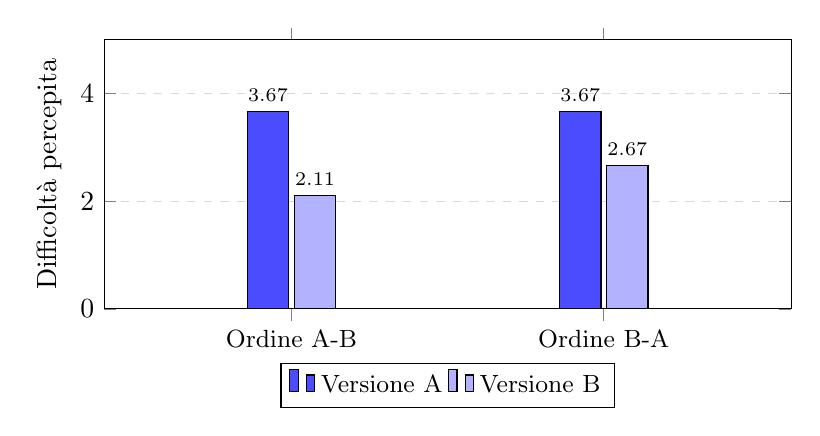
\begin{tikzpicture}
		\begin{axis}[
				ybar,
				bar width=15pt,
				width=0.85\textwidth,
				height=5cm,
				symbolic x coords={Ordine A-B, Ordine B-A},
				xtick=data,
				x tick label style={font=\small},
				ylabel={Difficoltà percepita},
				ymin=0, ymax=5,
				ymajorgrids=true,
				grid style={dashed, gray!30},
				enlarge x limits=0.6,
				legend style={at={(0.5,-0.2)}, anchor=north, legend columns=-1, font=\small},
				nodes near coords,
				every node near coord/.append style={font=\scriptsize, color=black},
			]
			\addplot+[
				fill=blue!70,
				draw=black
			] coordinates {
					(Ordine A-B,3.67)
					(Ordine B-A,3.67)
				};
			\addplot+[
				fill=blue!30,
				draw=black
			] coordinates {
					(Ordine A-B,2.11)
					(Ordine B-A,2.67)
				};
			\legend{Versione A, Versione B}
		\end{axis}
	\end{tikzpicture}
	\caption{Confronto della difficoltà percepita tra Versione A e Versione B per S1 in base all'ordine di esecuzione.}
	\label{fig:6-s1-2}
\end{figure}
